\documentclass[12pt,fleqn]{article}\usepackage{../../common}
\begin{document}
Direk Direngenlik Metotu (Direct Stiffness Method)

Bir yay sistemini temsil edebilecek direngenlik matrisini nasıl
bulabileceğimizin bir örneğini [2]'de gördük. Alternatif bir
teknik olarak üstdüşüm / üst üste koyma (superposition) tekniğini
işleyelim [1, sf. 38]. 

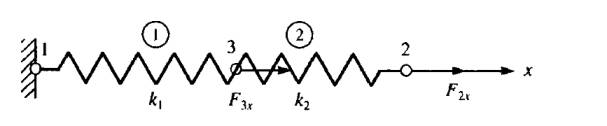
\includegraphics[width=20em]{compscieng_bpp35stiff01_01.jpg}


$$
\begin{array}{cc} & \begin{array}{ccc} a & b & c \end{array} \\ &
\left(
\begin{array}{ccc}
.1 & .1 & 0 \\
.4 & 1 & 0 \\
.8 & 0 & .4
\end{array}
\right)
\end{array}
$$

Kaynaklar

[1] Logan, {\em A First Course in the Finite Element Method}

[2] Bayramlı, {\em Hesapsal Bilim, Ders 1-8}

\end{document}
